\begin{figure}
\centering

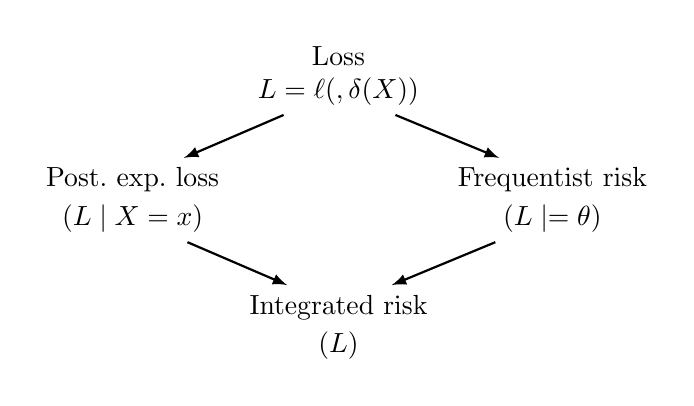
\begin{tikzpicture}[>=latex] %,text height=1.5ex,text depth=0.25ex]
  \matrix[row sep=-0.5ex,column sep=1ex] {
    & \node (Lt) {Loss}; &  \\
    & \node (L) {$L=\ell(\btheta,\delta(X))$}; &  \\
    & \node (blank1) {}; & \\
    & \node (blank2) {}; & \\
    & \node (blank3) {}; & \\
    & \node (blank4) {}; & \\
    \node (Bt) {Post.\ exp.\ loss}; & & \node (Rt) {Frequentist risk~}; \\ 
    \node (B) {$\E(L\mid X=x)$}; & & \node (R) {$\E(L\mid\btheta=\theta)$}; \\ 
    & \node (blank5) {}; & \\
    & \node (blank6) {}; & \\
    & \node (blank7) {}; & \\
    & \node (blank8) {}; & \\
    & \node (rt) {Integrated risk}; &  \\
    & \node (r) {$\E(L)$}; &  \\
    };
    
    % The diagram elements are now connected through arrows:
    \path[->]
        (L) edge[thick] (Bt)
        (L) edge[thick] (Rt)
        (B) edge[thick] (rt)
        (R) edge[thick] (rt)
;
\end{tikzpicture}

\caption{Visualizing the relationships between different decision-theoretic objects.}
\label{figure:diagram}
\end{figure}